\chapter{Модель водоплавающиего недеформируемого рыбоподобного робота}\label{ch:ch6}

\section{Описание конструкции водоплавающиего недеформируемого рыбоподобного робота}

Робот представляет собой полый объект, в продольном сечении имеющий форму профиля крыла NACA 0040 (см. рисунок \ref{Photo_NACA}) длиной 340 мм, шириной 134 мм. Высота робота 80 мм. Корпус изготовлен на 3Д-принтере из PLA-пластика, толщина стенки -- 2 мм. Внутри корпуса закреплен ротор с двигателем таким образом, что центр масс всей системы находится максимально близко к нижней грани робота. В качестве двигателя использовался мотор-редуктор фирмы Pololu с энкодером. Для передачи вращения с двигателя к ротору использовалась пара шестерен с передаточным отношением 3.5:1. Внутри так же располагается элемент питанияи плата с микроконтроллером модели STM32F303K8, управляющим вращением двигателем постоянного тока. Для управления двигателем используется драйвер двигателя постоянного тока VNH3SP30 фирмы STMicroelectronics. Энкодер использовался для определения положения ротора в течение экспериментов. Дифференцируя данные, полученные с энкодера, можно получить угловую скорость вращения ротора.
%Характеристики двигателя: номинальное напряжение питания -- 6 В, передаточное отношение редуктора -- 47:1, момент на валу -- 0.459 Нм, максимальная скорость вращения -- 120 об/мин. 


\begin{figure}[h]
	\centering
	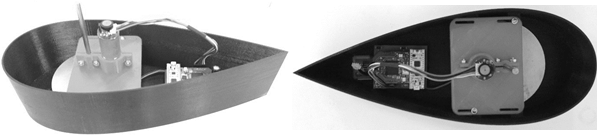
\includegraphics[width=1\linewidth]{Photo_NACA.png}%
	\caption{Безвинтовой рыбоподобный робот}
	\label{Photo_NACA}
\end{figure}

Реальная модель робота имеет следующие характеристики: m = $0.905$ кг; $I_0$ = $0.00844$ кг$\cdot$м2; Ротор изготовлен из алюминия, имеет внешний диаметр 110 мм, высоту 12 мм. Масса ротора $m_r$ = $0.327$ кг; момент инерции ротора $I_r$ = $0.00058$ кг$\cdot$м2. Конструкция робота позволяет смещать центр вращения ротора.

Управление осуществляется с персонального компьютера, для которого было разработано специальное программное обеспечение. Все команды роботу передаются по беспроводному каналу связи, используя Bluetooth.


\section{Описание системы управления водоплавающиего недеформируемого рыбоподобного робота}


\clearpage